% Fuller scientific draft. JOSS submission is ultimately paper.md, not LaTeX.
\documentclass[11pt]{article}
\usepackage[margin=1in]{geometry}
\usepackage[T1]{fontenc}
\usepackage{lmodern}
\usepackage{microtype}
\usepackage{amsmath}
\usepackage{graphicx}
\usepackage{hyperref}
\usepackage{placeins}
\usepackage[acronym,toc]{glossaries}
\hypersetup{colorlinks=true, allcolors=blue}
\setlength{\parindent}{0pt}
\glsdisablehyper

\newacronym{api}{API}{application programming interface}
\newacronym{ci}{CI}{continuous integration}
\newacronym{doi}{DOI}{digital object identifier}
\newacronym{mc}{MC}{Metropolis Monte Carlo}
\newacronym{py}{PY}{Percus--Yevick}
\newacronym{pypi}{PyPI}{Python Package Index}
\newacronym{rsa}{RSA}{random sequential addition}
\newacronym{rms}{RMS}{root-mean-square}

\title{PackLab: reproducible Percus--Yevick correlations for hard-sphere mixtures}
\author{Martin Poinsinet de Sivry-Houle, Xavier Attendu, Ton G. van Leeuwen, and Edwin van der Pol}
\date{}

\begin{document}
\maketitle

\begin{abstract}
PackLab is an open-source Python package centred on the analytical \gls{py} solution for multicomponent hard-sphere mixtures. %
It evaluates equilibrium-reference partial pair correlations and structure factors with unit-aware inputs and explicit Fourier-resolution diagnostics. %
A comparison with digitised \gls{py} curves from Tsang et al. demonstrates the matched binary-mixture workflow. %
Compiled \gls{rsa} and \gls{mc} tools are included as complementary add-ons for constructing non-overlapping configurations and sampling fixed-volume hard-sphere states; neither is treated as interchangeable with the analytical model. %
\end{abstract}

\section{Statement of need}

Hard-sphere models are useful idealisations for colloids, particulate materials, porous media, and disordered optical systems \cite{HansenMcDonald2013,Torquato2002}. %
Researchers often need a rapid, reproducible reference for mixture correlation functions or structure factors while exploring radius distributions, compositions, and volume fractions. %
These calculations are frequently implemented as disconnected scripts, which makes it easy to mix incompatible inputs, units, or Fourier-grid settings. %

Dependent-scattering calculations for dense, polydisperse suspensions provide a concrete example of this need. %
Attendu et al. combine single-particle Mie theory with a multicomponent \gls{py} hard-sphere model to predict the scattering properties of Intralipid across wavelength and concentration \cite{Attendu2026}. %
Such applications require the particle-size distribution, mixture correlation model, and numerical settings to remain internally consistent. %

PackLab provides these capabilities in one documented Python interface. %
Its core \texttt{analytical} namespace evaluates the \gls{py} hard-sphere-mixture reference \cite{Percus1958,Lebowitz1964}, preserving the mixture definition, dimensional inputs, and Fourier-resolution choices alongside the result. %
The Monte-Carlo namespace is complementary: it supplies reproducible \gls{rsa} configurations for coordinate-based downstream calculations and \gls{mc} relaxation at fixed particle count and radii. %
The package is intended for analytical parameter sweeps, structure-aware scattering models, and carefully interpreted comparisons between explicit configurations and an equilibrium hard-sphere reference. %

\section{Scientific scope}

\subsection{Percus--Yevick hard-sphere mixtures}

The analytical workflow evaluates the multicomponent \gls{py} approximation for hard-sphere mixtures. %
\texttt{PercusYevickDomain} converts radii, number fractions, and total volume fraction into species densities. %
\texttt{PercusYevickSolver} then evaluates partial pair correlations $g_{ij}(r)$ and structure factors on a user-supplied or automatically constructed wavenumber grid. %

\gls{py} is an approximate equilibrium reference. Its approximation error depends on mixture density, composition, and size ratio, while its numerical error depends separately on the inverse-transform grid. %
PackLab exposes both choices: automatic grids provide a documented default and the grid-construction interface permits explicit resolution studies. %
The digitised binary-mixture \gls{py} curves of Tsang et al. \cite{Tsang2001}, used in Figure~\ref{fig:tsang-comparison}, provide an external visual comparison at matched radii and partial volume fractions. %

\subsection{Configuration-generation add-ons}

\subsubsection{Random sequential addition}

\gls{rsa} proposes one sphere at a time. %
For a candidate centre $\mathbf{x}_i$ and radius $a_i$, PackLab accepts the candidate only if
\begin{equation}
	\lVert \mathbf{x}_i - \mathbf{x}_j \rVert \geq a_i + a_j
\end{equation}
for every previously accepted sphere $j$. %
Periodic simulations use the minimum-image convention. %
For a domain with volume $V$, the realised packing fraction is
\begin{equation}
	\phi = \frac{1}{V}\sum_i \frac{4\pi a_i^3}{3}. %
\end{equation}

\gls{rsa} is irreversible and history dependent: rejected candidates are discarded, and accepted spheres do not rearrange. %
It therefore does not sample an equilibrium hard-sphere fluid \cite{Feder1980}. %
PackLab makes this protocol explicit through independent stopping conditions, a stored random seed, periodic or finite domains, and constant, uniform, normal, log-normal, and discrete radius samplers. %
A spatial-neighbour grid limits overlap checks to nearby accepted spheres, preserving the \gls{rsa} acceptance rule while avoiding an all-pairs test for every proposal. %

\subsubsection{Metropolis Monte Carlo}

The \gls{mc} add-on takes a valid non-overlapping configuration, holds its particle count, radii, and class labels fixed, and proposes symmetric single-particle displacements. %
For hard spheres, a proposal is accepted exactly when it remains within the domain and introduces no overlap; this implements equilibrium sampling at fixed volume when burn-in, autocorrelation, and finite-size effects are assessed. %
\gls{rsa} can provide a convenient initial state, but its irreversible deposition history is not part of the subsequent \gls{mc} target distribution. %
The polydisperse hard-sphere Monte-Carlo structure factors of Frenkel et al. \cite{Frenkel1986} remain a candidate higher-precision equilibrium benchmark, while the ensemble and physical inputs of Ding et al. \cite{Ding1992} would need to be matched before comparison. %

\section{Software design and functionality}

Performance-critical analytical and configuration kernels are implemented in C++20 and exposed as native Python extensions. %
The Python layer provides NumPy-compatible results, \texttt{TypedUnit}-based dimensional inputs, plotting helpers, type information, and executable examples. %
Native extensions are installed beside their public Python APIs, keeping imports such as \texttt{PackLab.monte\_carlo} and \texttt{PackLab.analytical} stable and discoverable. %

An analytical workflow consists of a \texttt{PercusYevickDomain} and \texttt{PercusYevickSolver}. %
Beginner-facing examples use \texttt{wavenumber="auto"}, which selects a zero-inclusive grid from the smallest particle radius and requested distance range. %
Users can instead supply a grid with \texttt{make\_wavenumber\_grid} when they need explicit control over radial resolution and Fourier sampling. %

For explicit configurations, an \gls{rsa} workflow combines a \texttt{PackingDomain}, a radius sampler, and \texttt{RSAOptions}; \texttt{RSASimulator.run()} returns a \texttt{PackingResult}. %
The result contains centres, radii, class labels, packing statistics, and total or partial pair-correlation estimates. %
\texttt{MetropolisSimulator} accepts such a configuration with \texttt{MetropolisOptions} and reports displacement-move acceptance statistics. %
For \gls{rsa} ensemble calculations, \texttt{PackingEstimator} reports mean and standard deviation of partial correlations and insertion, rejection, runtime, and realised-packing diagnostics. %

\begin{figure}[t]
	\centering
	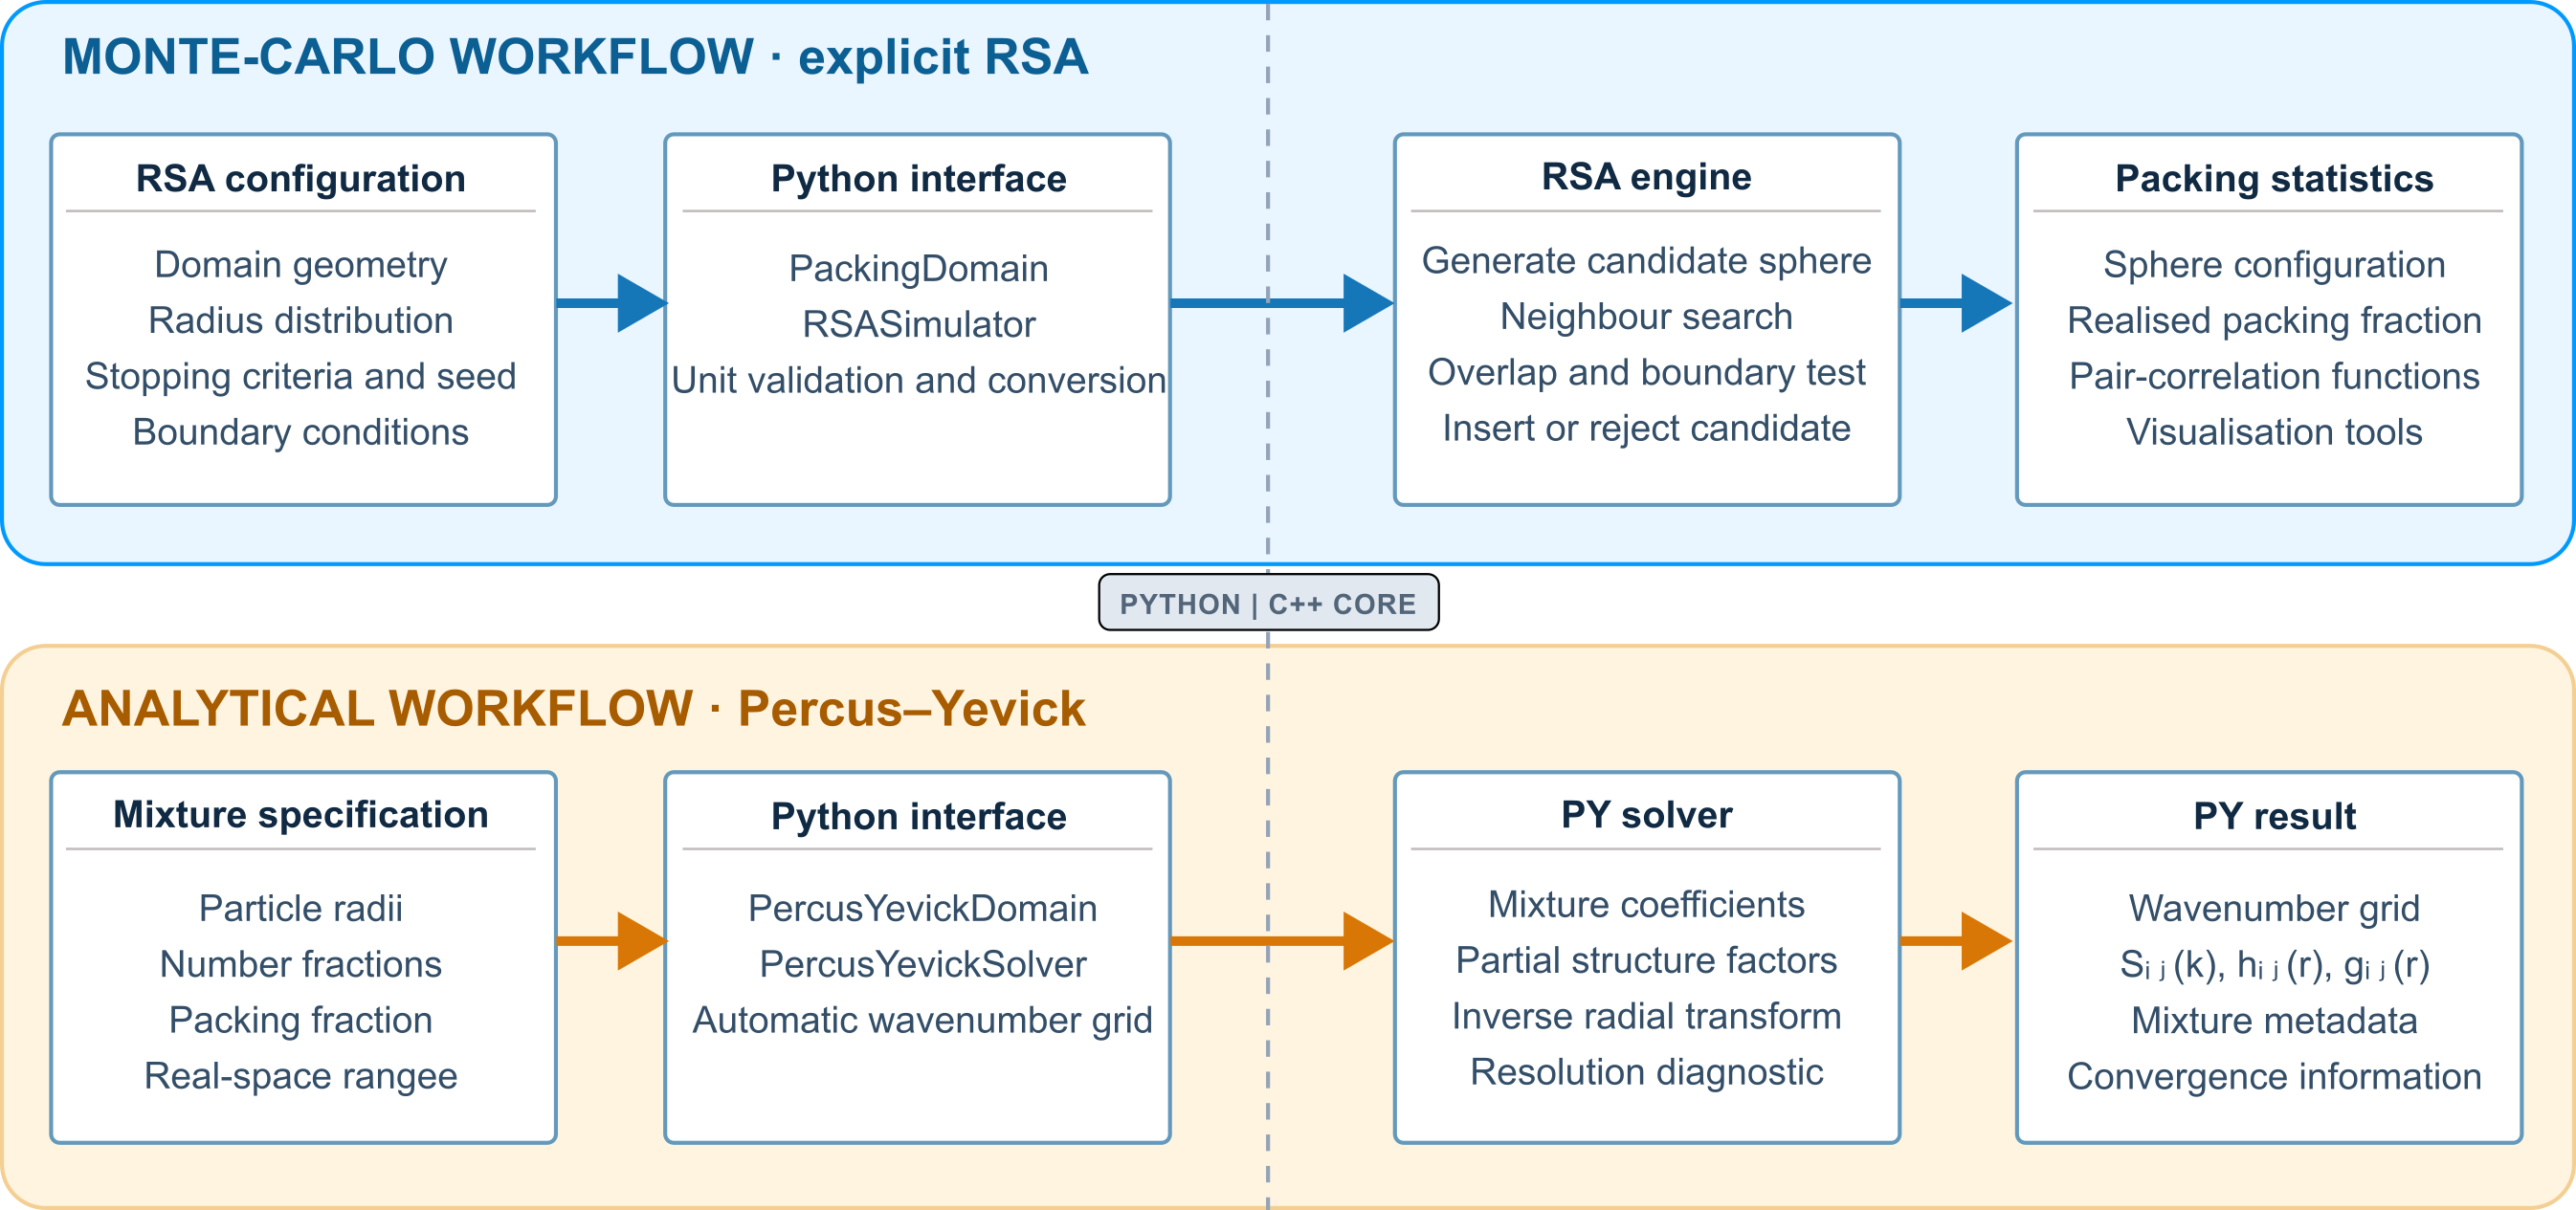
\includegraphics[width=\linewidth]{figures/architecture.png}
\caption{PackLab centres the \gls{py} equilibrium hard-sphere-mixture workflow and provides explicit-configuration add-ons. %
The analytical workflow evaluates pair correlations and structure factors for specified mixture inputs. %
The \gls{rsa} and \gls{mc} workflows create, respectively, irreversible deposition configurations and fixed-volume equilibrium samples. %
All workflows have unit-aware Python \glspl{api} backed by native C++ kernels, but their results are compared and interpreted rather than treated as interchangeable.}
	\label{fig:architecture}
\end{figure}

\section{Complementary configuration workflows}

Figure~\ref{fig:rsa} shows a fixed-seed periodic \gls{rsa} realisation of a binary mixture. %
The cross-section provides a direct geometric diagnostic of one generated configuration, while the correlation panel reports ensemble statistics for the same mixture. %
The example is generated entirely from the public \gls{api} and is included as an executable manuscript-figure script. %

\begin{figure}[t]
	\centering
	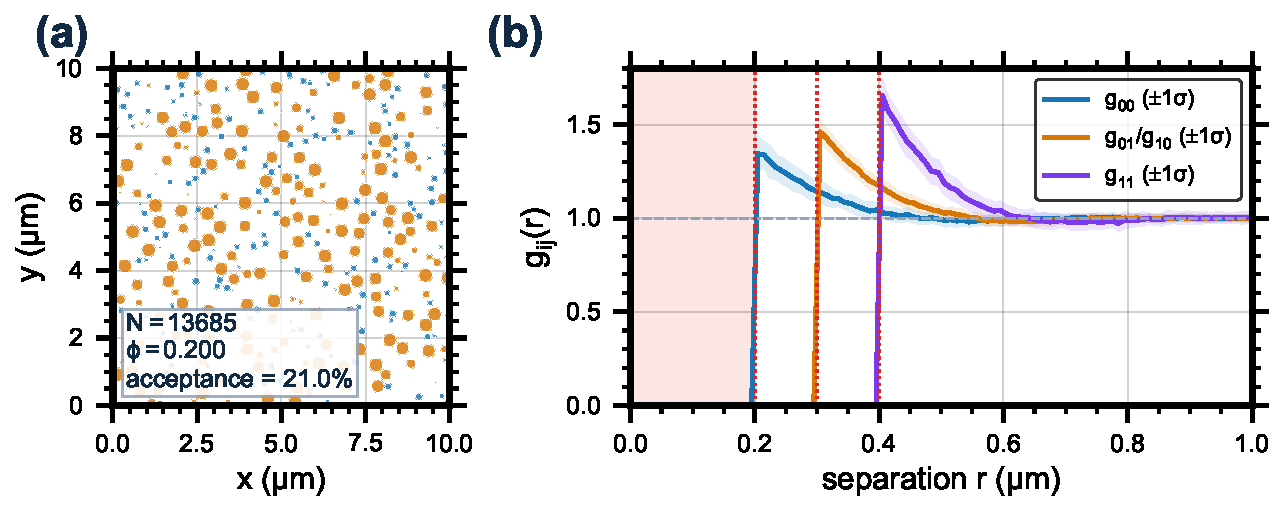
\includegraphics[width=\linewidth]{figures/figure2_rsa_example.pdf}
\caption{Reproducible periodic \gls{rsa} demonstration for a two-radius mixture. %
	The cubic domain has side length $10~\mathrm{\mu m}$; sphere radii are 100 and 200~nm with requested number fractions 0.65 and 0.35; the target packing fraction is 0.20; and the random seed is 20260828. %
	(a) Central cross-section of the accepted three-dimensional configuration, with colour indicating radius class. %
(b) The unique partial pair correlations, $g_{00}(r)$, $g_{01}(r)=g_{10}(r)$, and $g_{11}(r)$, estimated from 64 independent \gls{rsa} realisations. %
The legend identifies each ensemble-mean coloured line; its matching same-colour band shows $\pm1\sigma$, where $\sigma$ is the sample standard deviation across realisations. %
	The red shaded interval is the exclusion range shared by all pairs, while the red dotted lines mark the three contact separations, $0.20$, $0.30$, and $0.40~\mathrm{\mu m}$. %
	The dashed horizontal line marks the uncorrelated limit $g_{ij}(r)=1$.}
	\label{fig:rsa}
\end{figure}

\FloatBarrier

\section{Percus--Yevick validation and numerical resolution}

\subsection{Analytical correlation and structure-factor conventions}

For the \gls{rsa} estimator, used only for the complementary finite-configuration comparison below, $g_{ij}(r_b)$ is the ratio between the observed ordered $i$--$j$ pair count in radial shell $b$ and the ideal-gas expectation for the same configuration. %
For species counts $N_i$ and $N_j$, domain volume $V$, and shell volume $\Delta V_b$, the latter is
\begin{equation}
    E_{ij,b} = N_i\left(N_j-\delta_{ij}\right)\frac{\Delta V_b}{V},
    \qquad
    g_{ij}(r_b) = \frac{C_{ij,b}}{E_{ij,b}},
\end{equation}
where $\delta_{ij}$ is the Kronecker delta and $C_{ij,b}$ is the observed ordered count. %
The radial bins are spherical shells with centres $r_b=(b+1/2)\Delta r$ and extend to half the shortest box dimension; periodic estimates use minimum-image separations. %
When pair sampling is requested, the observed histogram is rescaled by the ratio of all unordered pairs to examined unordered pairs before this normalization. %

For the analytical workflow, $h_{ij}(r)=g_{ij}(r)-1$ and $H_{ij}(k)=\sqrt{\rho_i\rho_j}\,\tilde{h}_{ij}(k)$ is the density-scaled reciprocal-space total correlation. %
We use the corresponding density-scaled partial structure-factor convention
\begin{equation}
    S_{ij}(k)=\delta_{ij}+H_{ij}(k).
\end{equation}
This convention makes both the pair-correlation and structure-factor comparisons dimensionless and identifies the density factors required when transforming between them. %

The \gls{py} calculation uses an inverse radial Fourier transform, so its real-space result depends on wavenumber-grid extent and sampling density. %
For an isotropic mixture, the real-space total correlation is recovered from $H_{ij}(k)$ through
\begin{equation}
    h_{ij}(r) = \frac{1}{2\pi^2\sqrt{\rho_i\rho_j}}
    \int_0^\infty k^2 H_{ij}(k)\operatorname{sinc}(kr)\,\mathrm{d}k.
\end{equation}
At the maximum requested distance $r_{\max}$, the $\operatorname{sinc}(kr)$ factor has wavenumber period $2\pi/r_{\max}$, which is the most rapidly varying kernel over the requested distance range. %
A truncated grid omits high-wavenumber content, whereas a coarse grid under-samples oscillations in the sinc kernel. %
Either case can produce a visually smooth but numerically misleading correlation function. %

For \texttt{wavenumber="auto"}, PackLab uses a real-space resolution of one twentieth of the smallest radius and twelve samples per sinc-kernel oscillation at the maximum requested distance. %
When a user-provided grid has fewer than eight samples per oscillation, PackLab raises a runtime warning. %
These are numerical defaults, not physical constants, and the grid-construction \gls{api} allows stricter choices. %

\subsection{External binary-mixture comparison}

Figure~\ref{fig:tsang-comparison} is the manuscript's primary \gls{py} validation result. %
It compares PackLab's binary-mixture solution with manually digitised \gls{py} curves from Tsang et al. \cite{Tsang2001} at matched radius ratio and partial volume fractions. %
The expected hard-core contact locations, decay toward the uncorrelated limit, and damped post-contact structure agree visually across all three partial correlations. %
Because the reference was digitised from a printed plot, this is a reproducible visual validation rather than a high-precision error measurement. %

\begin{figure}[t]
    \centering
    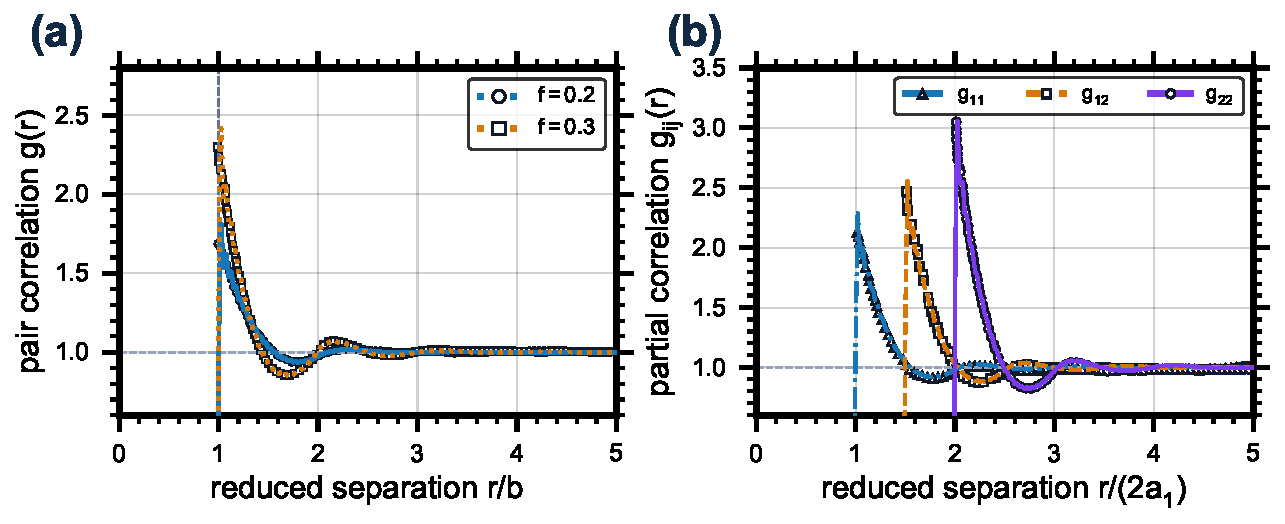
\includegraphics[width=\linewidth]{figures/figure4_independent_validation.pdf}
\caption{Book-style \gls{py} pair-correlation comparison based on Figures~8.1.3 and~8.3.4 of Tsang et al. \cite{Tsang2001}. %
(a) Mono-disperse reduced pair correlations at volume fractions $f=0.2$ and $f=0.4$, plotted against $r/b$. %
(b) Binary-mixture partial pair correlations against $r/(2a_1)$ for $a_2=2a_1$, partial volume fractions $f_1=0.2$ and $f_2=0.1$; colour-coded curves with distinct line styles are PackLab \gls{py} solutions, and black open triangle, square, and circle markers are manually digitised \gls{py} reference curves from Figure~8.3.4. %
The digitised markers provide a visual reference only: their precision is limited by extraction from the printed figure, and they do not replace the source numerical dataset.}
    \label{fig:tsang-comparison}
\end{figure}

\FloatBarrier

\subsection{Complementary RSA comparison and numerical convergence}

Figure~\ref{fig:validation} distinguishes model comparison from numerical verification. %
Panel (a) compares all unique partial correlations from a 100-realisation \gls{rsa} ensemble with \gls{py} evaluated for the same binary-mixture inputs and the same radial coordinates. %
It demonstrates how PackLab makes the common inputs, statistical uncertainty, and model-dependent differences inspectable. %
Panel (b) is the actual numerical convergence check: it measures the \gls{py} result against a separately specified, much finer wavenumber grid. %

\begin{figure}[t]
	\centering
	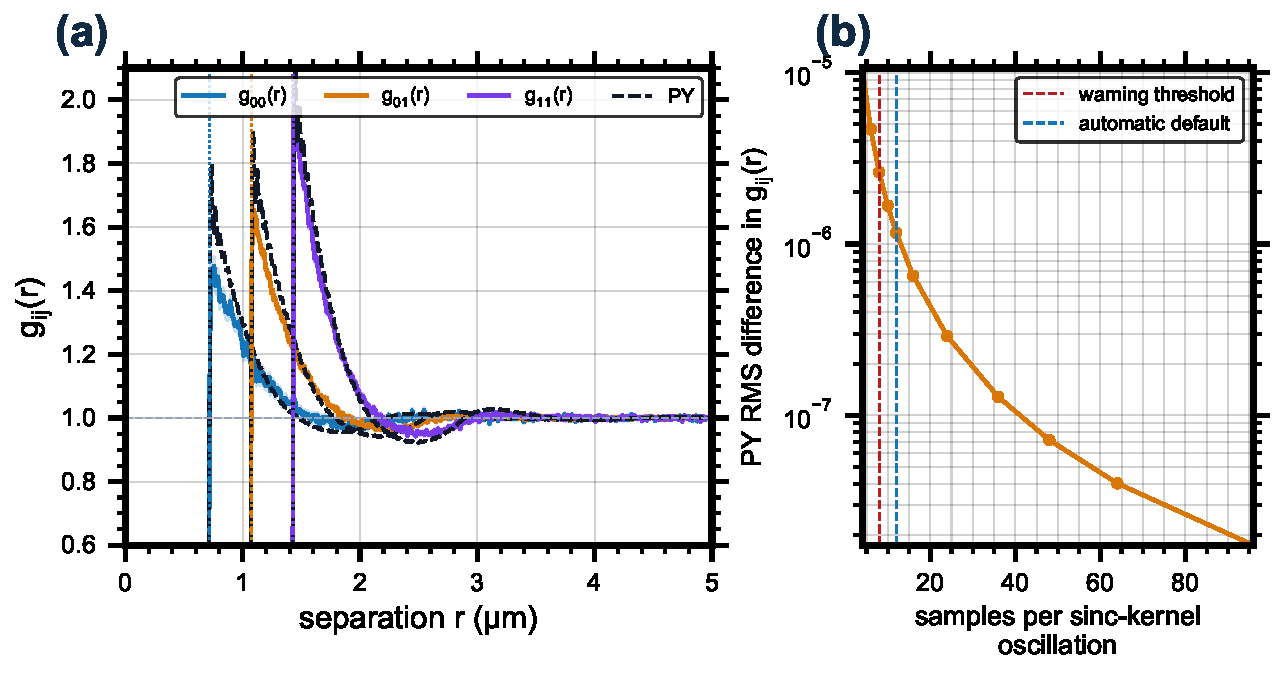
\includegraphics[width=\linewidth]{figures/figure3_validation.pdf}
\caption{Matched \gls{rsa}--\gls{py} comparison and \gls{py} numerical convergence for a binary mixture with radii 0.357 and 0.714~\textmu m, equal number fractions, and total volume fraction 0.25. %
(a) The coloured solid curves and black dashed curves show, respectively, the \gls{rsa} ensemble mean and the corresponding \gls{py} equilibrium reference for $g_{00}(r)$, $g_{01}(r)$, and $g_{11}(r)$. %
Same-colour bands show the \gls{rsa} one-standard-error uncertainty; dotted lines mark the corresponding hard-core contact distances, and the grey dashed line marks $g_{ij}(r)=1$. %
The principal short-range discrepancies are physical rather than numerical: \gls{rsa} is a finite, irreversible insertion protocol, whereas \gls{py} approximates an equilibrium hard-sphere mixture. %
The uncertainty bands quantify finite-ensemble variation, while panel (b) separately tests the inverse-transform grid error. %
(b) \gls{rms} difference between \gls{py} calculations and a separately specified 512-samples-per-oscillation reference as the wavenumber grid is refined. %
The red and blue dashed lines identify PackLab's under-resolution warning threshold (8 samples per oscillation) and automatic default (12), respectively. %
The decreasing error provides numerical-convergence evidence for the analytical calculation; physical validation of the \gls{py} approximation instead requires an independent equilibrium benchmark such as Frenkel et al. \cite{Frenkel1986}. A comparison with Ding et al. \cite{Ding1992} additionally requires matching its ensemble definition.}
	\label{fig:validation}
\end{figure}

\FloatBarrier

\section{Quality control, availability, and limitations}

PackLab includes public-\gls{api} tests for analytical hard-core exclusion, automatic-grid selection, grid warnings, and convergence against a refined reference, as well as samplers, packing validity, periodic boundaries, and Metropolis move validation. %
Executable documentation examples are organised around analytical, \gls{rsa}, \gls{mc}, and comparison workflows. %
\Gls{ci} builds the native extensions and runs the test suite for CPython 3.11--3.13. %

PackLab version 0.1.0 requires Python 3.10 or later, is released under the MIT License, and is available from \gls{pypi} and conda. %
Source code, documentation, issue tracking, and release history are available at \url{https://github.com/MartinPdeS/PackLab}. %
Release-specific citation metadata is maintained in \texttt{.zenodo.json}. %
The repository's v0.1.0 release is archived at \href{https://doi.org/10.5281/zenodo.20207810}{10.5281/zenodo.20207810}. %

The current scope is three-dimensional, spherical, hard-core particles in cuboidal domains. %
\gls{rsa} should not be interpreted as an equilibrium-fluid simulator; \gls{mc} requires explicit equilibration assessment; and \gls{py} should not be interpreted as a measured structure or a general interaction model. %

The practical limits of both workflows depend on the requested mixture and numerical settings. %
For \gls{rsa}, insertion becomes progressively less efficient as the requested packing fraction increases; finite domains, broad radius distributions, and stringent stopping conditions can prevent the requested target from being reached. %
Consequently, users should report the realised packing fraction, stopping diagnostics, random seed, ensemble size, and domain size rather than treating a requested target as an achieved state. %
Pair-correlation estimates from finite configurations additionally depend on binning and are subject to finite-size uncertainty, particularly near the largest separations accessible in a domain. %
For \gls{mc}, users should assess burn-in, autocorrelation, proposal acceptance, and finite-size effects before treating separated chain states as equilibrium samples. %

For \gls{py}, the approximation error depends on density, composition, and particle-size ratio, and is separate from Fourier-grid discretisation error. %
The automatic grid and under-resolution warning are useful safeguards, but they do not establish convergence for every mixture, especially when near-contact structure is sharp, size ratios are extreme, or correlations are required over a long distance range. %
Users should refine the wavenumber grid and compare against an independently chosen equilibrium benchmark when the analytical result informs a quantitative conclusion. %
PackLab's separate namespaces, explicit input definitions, recorded stochastic settings, and grid diagnostics are designed to make these limitations visible at the point of use. %

\section{Acknowledgements}

The author thanks the open-source scientific Python ecosystem and the users who provide feedback, issues, and reproducible examples. %

\clearpage
\bibliographystyle{plain}
\bibliography{references}
\end{document}
